\documentclass{beamer}
\mode<presentation>
\usepackage{amsmath}
\usepackage{amssymb}
\usepackage{bm}
%\usepackage{advdate}
\usepackage{adjustbox}
\usepackage{subcaption}
%\usepackage{enumitem}
\usepackage{enumerate}
\usepackage{multicol}
\usepackage{mathtools}
\usepackage{listings}
\usepackage{url}
\def\UrlBreaks{\do\/\do-}
\usetheme{Boadilla}
\usecolortheme{lily}
\setbeamertemplate{footline}
{
  \leavevmode%
  \hbox{%
  \begin{beamercolorbox}[wd=\paperwidth,ht=2.25ex,dp=1ex,right]{author in head/foot}%
    \insertframenumber{} / \inserttotalframenumber\hspace*{2ex} 
  \end{beamercolorbox}}%
  \vskip0pt%
}
\setbeamertemplate{navigation symbols}{}

\providecommand{\nCr}[2]{\,^{#1}C_{#2}} % nCr
\providecommand{\nPr}[2]{\,^{#1}P_{#2}} % nPr
\providecommand{\mbf}{\mathbf}
\providecommand{\pr}[1]{\ensuremath{\Pr\left(#1\right)}}
\providecommand{\qfunc}[1]{\ensuremath{Q\left(#1\right)}}
\providecommand{\sbrak}[1]{\ensuremath{{}\left[#1\right]}}
\providecommand{\lsbrak}[1]{\ensuremath{{}\left[#1\right.}}
\providecommand{\rsbrak}[1]{\ensuremath{{}\left.#1\right]}}
\providecommand{\brak}[1]{\ensuremath{\left(#1\right)}}
\providecommand{\lbrak}[1]{\ensuremath{\left(#1\right.}}
\providecommand{\rbrak}[1]{\ensuremath{\left.#1\right)}}
\providecommand{\cbrak}[1]{\ensuremath{\left\{#1\right\}}}
\providecommand{\lcbrak}[1]{\ensuremath{\left\{#1\right.}}
\providecommand{\rcbrak}[1]{\ensuremath{\left.#1\right\}}}
\providecommand{\rank}{\text{rank}}
\theoremstyle{remark}
\newtheorem{rem}{Remark}
\newcommand{\sgn}{\mathop{\mathrm{sgn}}}
\providecommand{\abs}[1]{\left\vert#1\right\vert}
\providecommand{\res}[1]{\Res\displaylimits_{#1}} 
\providecommand{\norm}[1]{\lVert#1\rVert}
\providecommand{\mtx}[1]{\mathbf{#1}}
\providecommand{\mean}[1]{E\left[ #1 \right]}
\providecommand{\fourier}{\overset{\mathcal{F}}{ \rightleftharpoons}}
%\providecommand{\hilbert}{\overset{\mathcal{H}}{ \rightleftharpoons}}
\providecommand{\system}{\overset{\mathcal{H}}{ \longleftrightarrow}}
	%\newcomamand{\solution}[2]{\vec{Solution:}{#1}}
%\newcommand{\solution}{\noindent \vec{Solution: }}
\providecommand{\dec}[2]{\ensuremath{\overset{#1}{\underset{#2}{\gtrless}}}}
\newcommand{\myvec}[1]{\ensuremath{\begin{pmatrix}#1\end{pmatrix}}}
\newenvironment{amatrix}[1]{%
  \left(\begin{array}{@{}*{#1}{c}|c@{}}
}{%
  \end{array}\right)
}
\let\vec\mathbf

\lstset{
%language=C,
frame=single, 
breaklines=true,
columns=fullflexible
}

%\numberwithin{equation}{section}

\title{Matgeo-q.2.7.8}
\author{AI25BTECH11036-SNEHAMRUDULA}

\date{\today} 
\begin{document}

\begin{frame}
\titlepage
\end{frame}

\section*{Outline}


\begin{frame}
\frametitle{Question}
2.7.8 Find $|\vec{a} \times \vec{b}|$, if 
$\vec{a} = 2\mathbf{i} + \mathbf{j} + 3\mathbf{k}$ and 
$\vec{b} = 3\mathbf{i} + 5\mathbf{j} - 2\mathbf{k}$.
\end{frame}
\begin{frame}
\frametitle{solution}

\[
|A_{23} \; B_{23}| = 
\begin{vmatrix}
1 & 3 \\
5 & -2
\end{vmatrix}
= (1)(-2) - (3)(5) = -17 \tag{2.7.8.1}
\]

\[
|A_{31} \; B_{31}| = 
\begin{vmatrix}
2 & 3 \\
3 & -2
\end{vmatrix}
= (2)(-2) - (3)(3) = -13 \tag{2.7.8.2}
\]

\[
|A_{12} \; B_{12}| = 
\begin{vmatrix}
2 & 1 \\
3 & 5
\end{vmatrix}
= (2)(5) - (1)(3) = 7 \tag{2.7.8.3}
\]

\[
\vec{a} \times \vec{b} =
\begin{vmatrix}
\mathbf{i} & \mathbf{j} & \mathbf{k} \\
2 & 1 & 3 \\
3 & 5 & -2
\end{vmatrix}
= (-17)\mathbf{i} - (-13)\mathbf{j} + (7)\mathbf{k} \tag{2.7.8.4}
\]

\[
\vec{a} \times \vec{b} = -17\mathbf{i} + 13\mathbf{j} + 7\mathbf{k}
\]

\[
|\vec{a} \times \vec{b}| = 
\sqrt{(-17)^2 + (13)^2 + (7)^2} 
= \sqrt{289 + 169 + 49} 
= \sqrt{507} 
= 13\sqrt{3} 
\]

\[
\boxed{|\vec{a} \times \vec{b}| = 13\sqrt{3}}
\]

\end{frame}
    \begin{frame}{Graphical Representation}
   \begin{figure}[h!]
\centering
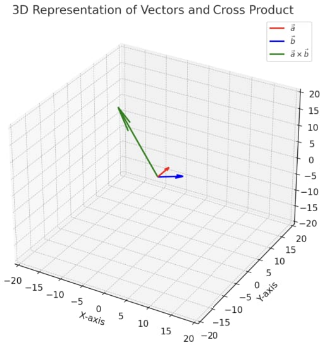
\includegraphics[width=0.5\linewidth]{fig2.7.8}

\end{figure}
\end{frame}



\end{document}